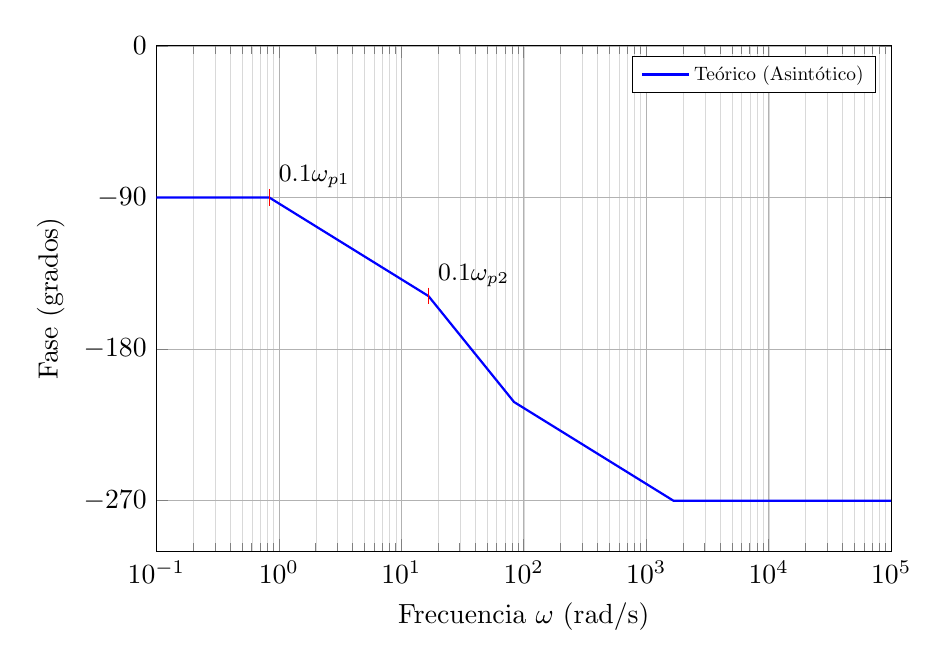
\begin{tikzpicture}
\begin{semilogxaxis}[
    xlabel={Frecuencia $\omega$ (rad/s)},
    ylabel={Fase (grados)},
    grid=both,
    grid style={line width=.1pt, draw=gray!30},
    major grid style={line width=.2pt, draw=gray!60},
    xmin=1e-1, xmax=1e5,
    ymin=-300, ymax=0,
    ytick={0, -90, -180, -270},
    width=0.9\columnwidth,
    height=8cm,
    legend style={
    nodes={scale=0.7, transform shape}
}
]

\addplot[thick, blue] coordinates {
    (0.1, -90)
    (0.8333, -90)
    (16.667, -148.54)
    (83.333, -211.44)
    (1666.667, -270)
    (1e5, -270)
};
\addlegendentry{Teórico (Asintótico)}

\addplot[mark=|, mark size=3pt, red, forget plot] coordinates {(0.8333, -90)};
\node[anchor=south west, font=\small, text=black] at (axis cs:0.8333, -90) {$0.1\omega_{p1}$};

\addplot[mark=|, mark size=3pt, red, forget plot] coordinates {(16.667, -148.54)};
\node[anchor=south west, font=\small, text=black] at (axis cs:16.667, -148.54) {$0.1\omega_{p2}$};

% TODO: Descomentar e indicar el path correcto al archivo exportado de LTSpice
% \addplot[thick, dashed, orange] table [
%     skip first n=1,
%     x expr=\thisrowno{0} * 2 * pi,
%     y index=2
% ] {sources/bode_3_real.txt};
% \addlegendentry{Simulación LTSpice}

\end{semilogxaxis}
\end{tikzpicture}
